\documentclass[12pt,a4paper]{article}
\usepackage{task}

\newcommand{\contestName}{Olympiad in Informatics 20YY}
\newcommand{\contestDates}{Month 1 -- 8 20YY}
\newcommand{\contestPlace}{The place}
\newcommand{\contestRound}{Contest...}
\newcommand{\statementLanguage}{English (Official)}
\newcommand{\taskShortName}{__TPARAM_SHORT_NAME__}


\begin{document}



% Tex fragment for task statement headers
% Usage:
%       % Defining parameters required for header
%       \newcommand{\contestName}{Name of the Contest Series}
%       \newcommand{\contestDates}{Month 1 -- 8 20XX}
%       \newcommand{\contestPlace}{City, Country}
%       \newcommand{\contestRound}{Day 1}
%       \newcommand{\statementLanguage}{en (US)}
%       \newcommand{\taskShortName}{task_short_name}
%       

% Tex fragment for task statement headers
% Usage:
%       % Defining parameters required for header
%       \newcommand{\contestName}{Name of the Contest Series}
%       \newcommand{\contestDates}{Month 1 -- 8 20XX}
%       \newcommand{\contestPlace}{City, Country}
%       \newcommand{\contestRound}{Day 1}
%       \newcommand{\statementLanguage}{en (US)}
%       \newcommand{\taskShortName}{task_short_name}
%       

% Tex fragment for task statement headers
% Usage:
%       % Defining parameters required for header
%       \newcommand{\contestName}{Name of the Contest Series}
%       \newcommand{\contestDates}{Month 1 -- 8 20XX}
%       \newcommand{\contestPlace}{City, Country}
%       \newcommand{\contestRound}{Day 1}
%       \newcommand{\statementLanguage}{en (US)}
%       \newcommand{\taskShortName}{task_short_name}
%       \input{header.tex}
%


%--------------------- tools ----------------------
\makeatletter
% \expandafter for the case that the parameter is given in a command
\newcommand{\escapeUnderscores}[1]{\expandafter\@repl@underscores#1_\relax}
\def\@repl@underscores#1_#2\relax{%
    \ifx \relax #2\relax
        % #2 is empty => finish
        #1%
    \else
        % #2 is not empty => underscore was contained, needs to be replaced
        #1%
        \textunderscore
        % continue replacing
        % #2 ends with an extra underscore so I don't need to add another one
        \@repl@underscores#2\relax
    \fi
}
\makeatother
% -------------------------------------------------

\vspace*{-3em}\hspace*{-.5cm}
\begin{tabular}{ccl}
    \hspace{1mm}
\includegraphics[width=2.5cm]{logo.png}
    & 
    \begin{minipage}[b]{10cm}
        \setlength{\baselineskip}{1.05\baselineskip}
        \sffamily
        \makebox[0pt][l]{\bfseries \large \contestName}  \\
        \contestDates \\ 
        \contestPlace
    \end{minipage}
    & 
    \begin{minipage}[b]{3.7cm}
        \begin{flushright}
            \makebox[0pt][r]{\ttfamily \bfseries \large \escapeUnderscores{\taskShortName}}  \\[.2em]
            \sffamily
            \contestRound \\
            \statementLanguage
        \end{flushright}
    \end{minipage}
\end{tabular} 
\hrule height .06em

%


%--------------------- tools ----------------------
\makeatletter
% \expandafter for the case that the parameter is given in a command
\newcommand{\escapeUnderscores}[1]{\expandafter\@repl@underscores#1_\relax}
\def\@repl@underscores#1_#2\relax{%
    \ifx \relax #2\relax
        % #2 is empty => finish
        #1%
    \else
        % #2 is not empty => underscore was contained, needs to be replaced
        #1%
        \textunderscore
        % continue replacing
        % #2 ends with an extra underscore so I don't need to add another one
        \@repl@underscores#2\relax
    \fi
}
\makeatother
% -------------------------------------------------

\vspace*{-3em}\hspace*{-.5cm}
\begin{tabular}{ccl}
    \hspace{1mm}
\includegraphics[width=2.5cm]{logo.png}
    & 
    \begin{minipage}[b]{10cm}
        \setlength{\baselineskip}{1.05\baselineskip}
        \sffamily
        \makebox[0pt][l]{\bfseries \large \contestName}  \\
        \contestDates \\ 
        \contestPlace
    \end{minipage}
    & 
    \begin{minipage}[b]{3.7cm}
        \begin{flushright}
            \makebox[0pt][r]{\ttfamily \bfseries \large \escapeUnderscores{\taskShortName}}  \\[.2em]
            \sffamily
            \contestRound \\
            \statementLanguage
        \end{flushright}
    \end{minipage}
\end{tabular} 
\hrule height .06em

%


%--------------------- tools ----------------------
\makeatletter
% \expandafter for the case that the parameter is given in a command
\newcommand{\escapeUnderscores}[1]{\expandafter\@repl@underscores#1_\relax}
\def\@repl@underscores#1_#2\relax{%
    \ifx \relax #2\relax
        % #2 is empty => finish
        #1%
    \else
        % #2 is not empty => underscore was contained, needs to be replaced
        #1%
        \textunderscore
        % continue replacing
        % #2 ends with an extra underscore so I don't need to add another one
        \@repl@underscores#2\relax
    \fi
}
\makeatother
% -------------------------------------------------

\vspace*{-3em}\hspace*{-.5cm}
\begin{tabular}{ccl}
    \hspace{1mm}
\includegraphics[width=2.5cm]{logo.png}
    & 
    \begin{minipage}[b]{10cm}
        \setlength{\baselineskip}{1.05\baselineskip}
        \sffamily
        \makebox[0pt][l]{\bfseries \large \contestName}  \\
        \contestDates \\ 
        \contestPlace
    \end{minipage}
    & 
    \begin{minipage}[b]{3.7cm}
        \begin{flushright}
            \makebox[0pt][r]{\ttfamily \bfseries \large \escapeUnderscores{\taskShortName}}  \\[.2em]
            \sffamily
            \contestRound \\
            \statementLanguage
        \end{flushright}
    \end{minipage}
\end{tabular} 
\hrule height .06em


\section*{__TPARAM_TASK_TITLE__}

Here we go.

\begin{center}
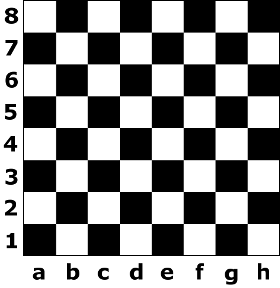
\includegraphics[width=.5\textwidth]{board.png}
\end{center}

\subsection*{Implementation details}

You should implement the following procedure.
It will be called by the grader once for each test case.

\begin{prog}
int __TPARAM_GRADER_FUNCTION_NAME__(int n)
\end{prog}

\begin{itemize}
    \item $n$: ...
    \item This procedure should return ...
\end{itemize}


\subsection*{Examples}

\subsubsection*{Example 1}

Consider $n=5$.

\begin{prog}
__TPARAM_GRADER_FUNCTION_NAME__(5)
\end{prog}

The answer is $0$ because...

\subsection*{Constraints}

\begin{itemize}
    \item $1 \leq n \leq  1000$
\end{itemize}

\subsection*{Subtasks}

\begin{enumerate}
    \item (20 points) $n \leq 100$,
    \item (80 points) No additional constraints.
\end{enumerate}

\subsection*{Sample grader}

The sample grader reads the input in the following format:
\begin{itemize}
    \item line $1$:  $\;\;n$
\end{itemize}

The sample grader prints a single line containing the return value of \code{__TPARAM_GRADER_FUNCTION_NAME__}.

\end{document}
